% !TEX encoding = UTF-8 Unicode
%%%%%%%%%%%%%%%%%%%%%%%%%%%%%%%%%%%%%%%%%
% Journal Article
% LaTeX Template
% Version 1.4 (15/5/16)
%
% This template has been downloaded from:
% http://www.LaTeXTemplates.com
%
% Original author:
% Frits Wenneker (http://www.howtotex.com) with extensive modifications by
% Vel (vel@LaTeXTemplates.com)
%
% License:
% CC BY-NC-SA 3.0 (http://creativecommons.org/licenses/by-nc-sa/3.0/)
%
%%%%%%%%%%%%%%%%%%%%%%%%%%%%%%%%%%%%%%%%%

%----------------------------------------------------------------------------------------
%	PACKAGES AND OTHER DOCUMENT CONFIGURATIONS
%----------------------------------------------------------------------------------------
\documentclass[oneside, 11 pt]{article}
\usepackage[utf8]{inputenc}
\usepackage[T1]{fontenc}
\usepackage{textcomp}
\usepackage[portuguese]{babel}
\usepackage{blindtext} % Package to generate dummy text throughout this template 
\usepackage{comment}
\usepackage{listings}
\usepackage{xcolor}

\usepackage{hyperref} % For hyperlinks in the PDF

\usepackage{inconsolata}
\lstset{
	language=bash, %% Troque para PHP, C, Java, etc... bash é o padrão
	basicstyle=\ttfamily\small,
	numberstyle=\footnotesize,
	backgroundcolor=\color{gray!10},
	frame=single,
	tabsize=2,
	rulecolor=\color{black!30},
	escapeinside={\%*}{*)},
	breaklines=true,
	breakatwhitespace=true,
	framextopmargin=2pt,
	framexbottommargin=2pt,
	inputencoding=utf8,
	extendedchars=true,
	literate={á}{{\'a}}1 {ã}{{\~a}}1 {é}{{\'e}}1 {í}{{\'i}}1,
}
\usepackage[hmarginratio=1:1,top=32mm,columnsep=20pt]{geometry} % Document margins
\usepackage[hang, small,labelfont=bf,up,textfont=it,up]{caption} % Custom captions under/above floats in tables or figures
\usepackage{booktabs} % Horizontal rules in tables

\usepackage{lettrine} % The lettrine is the first enlarged letter at the beginning of the text

\usepackage{enumitem} % Customized lists
\setlist[itemize]{noitemsep} % Make itemize lists more compact

\usepackage{titlesec} % Allows customization of titles
%\renewcommand\thesection{\Roman{section}} % Roman numerals for the sections
%\renewcommand\thesubsection{\roman{subsection}} % roman numerals for subsections
\titleformat{\section}[block]{\large\scshape\centering}{\thesection.}{1em}{} % Change the look of the section titles
\titleformat{\subsection}[block]{\large}{\thesubsection.}{1em}{} % Change the look of the section titles

\usepackage{fancyhdr} % Headers and footers
\pagestyle{fancy} % All pages have headers and footers
\fancyhead{} % Blank out the default header
\fancyhead[C]{Introdução ao Bash - Comandos e Scripts} % Custom header text

\usepackage{titling} % Customizing the title section

\usepackage{graphicx}
\usepackage{float}
\renewcommand{\arraystretch}{1.5}
\usepackage{multirow}
\setlength{\parindent}{18pt}
\setcounter{secnumdepth}{0}

\usepackage{xcolor}
\hypersetup{
	colorlinks,
	linkcolor={red!60!black},
	citecolor={blue!50!black},
	urlcolor={blue!80!black}
}
%----------------------------------------------------------------------------------------
%	TITLE SECTION
%----------------------------------------------------------------------------------------

\setlength{\droptitle}{-4\baselineskip} % Move the title up

\pretitle{\begin{center}\Huge\bfseries} % Article title formatting
	\posttitle{\end{center}} % Article title closing formatting
\title{Introdução ao Bash} % Article title
\author{%
	\textsc{Guilherme Bittencourt Bueno da Silva} \\[1ex] % Your name
	\normalsize Universidade Federal do Paraná \\ % Your institution
	\normalsize {gbbs14@inf.ufpr.br} % Your email address
	%\and % Uncomment if 2 authors are required, duplicate these 4 lines if more
	%\textsc{Jane Smith}\thanks{Corresponding author} \\[1ex] % Second author's name
	%\normalsize University of Utah \\ % Second author's institution
	%\normalsize \href{mailto:jane@smith.com}{jane@smith.com} % Second author's email address
}
\date{\today} % Leave empty to omit a date
\renewcommand{\maketitlehookd}{%
	
	%\begin{abstract}
	%\noindent \blindtext % Dummy abstract text - replace \blindtext with your abstract text
	%\end{abstract}
}

%----------------------------------------------------------------------------------------

\begin{document}
	
	% Print the title
	\maketitle
	
	\tableofcontents
	%----------------------------------------------------------------------------------------
	%	ARTICLE CONTENTS
	%----------------------------------------------------------------------------------------
	\section{Resumo}
	 O Shell é uma interface eficiente de acesso aos serviços do kernel. Shells mais recentes permitem operações além da simples interpretação de comandos e facilitam o uso com funcionalidades que automatizam tarefas repetitivas, porém, o custo dessa facilidade é uma interface pouco intuitiva, por isso, esse material explica brevemente a história e a estrutura do shell e apresenta as funcionalidades do Bash, o Shell padrão na maioria das distribuições Linux.
	
	\section{Introdução}
	Computadores são imprescindíveis em  diversas áreas de aplicação, possuíndo formas específicas para cada tipo de aplicação. Para que os computadores sejam amplamente acessíveis, eles possuem uma quantidade imensa de interfaces para que um usuário sem nenhum conhecimento seja capaz de utilizar um computador. Uma interface, em ciência da computação, é a fronteira que define a forma de comunicação entre duas entidades. Ela pode ser entendida como uma abstração que estabelece a forma de interação da entidade com o mundo exterior, através da separação dos métodos de comunicação externa dos detalhes internos da operação \cite{interface}. Existem interfaces em vários níveis, como interfaces gráficas para que usuários básicos possam selecionar aplicações, ou interfaces das próprias aplicações que permitem que o usuário faça uso do computador através de abstrações.
	
	O Shell é uma interface entre o usuário e o sistema operacional (SO), usada para simplificar o uso desse, escondendo detalhes específicos de cada versão do SO. Diferente das interfaces citadas acima, o Shell é direcionado a um público menos abrangente e não possui um sistema de apontar e clicar (que é mais lento e repetitivo que uma interface textual). A intenção dessa interface não é de facilitar o aprendizado para usuários iniciantes, e sim de facilitar e otimizar as tarefas de usuários que utilizam constantemente o sistema. Por isso, é necessário (ou, ao menos, muito importante) o uso de um material como este para aprender a usar o Shell da maneira correta, eliminando a redigitação e aproveitando ao máximo os recursos oferecidos.
	
	Quando foi criado, o Shell era a interface padrão de acesso ao computador, e nessa época, os SOs apenas tratavam do gerenciamento de processos e da memória, sem incluir aplicações e interfaces adicionais, então, para o usuário (ou, para os operadores do mainframe) escolher um bom Shell era tão importante quanto escolher um SO.
	
	Com o avanço da tecnologia, a maneira de interagir com um computador mudou tanto que muitos usuários não precisam saber o que é um shell, a maioria dos usuários, nem precisam utilizar um shell.	Considerando que há 30 anos atrás, os usuários só tinham acesso ao mainframe através de uma estação com teclado e monitor para utilizar os comandos do shell, é possível dizer que hoje, computador é algo completamente diferente. Porém, hoje em dia, ainda usamos os mesmos termos para definir partes do sistema que hoje funcionam de maneira diferente. Então antes de apresentar a história do Shell, é bom diferenciar conceitos que são facilmente confundidos.
	
	\part{Introdução ao Shell}
	\section{Terminal vs Console vs Shell}
	
	\subsection{Terminal}
	Se você usa alguma distribuição UNIX, provavelmente já deve ter usado um terminal, mas certamente, não da mesma maneira que terminais eram utilizados antigamente. É fácil confundir e achar que o terminal está executando as operações, mas na verdade o terminal é apenas uma interface gráfica de um console. Pensando no terminal de antigamente é mais fácil entender que não é o terminal que executa os comandos. O terminal era algo físico, um ponto de acesso com meios de entrada e saída (teclado e monitor) para iteragir com a máquina, pois antes um computador era compartilhado por vários operadores.
	Atualmente, cada usuário utiliza uma máquina diferente, e isso é um terminal:
	\begin{figure}[h]
		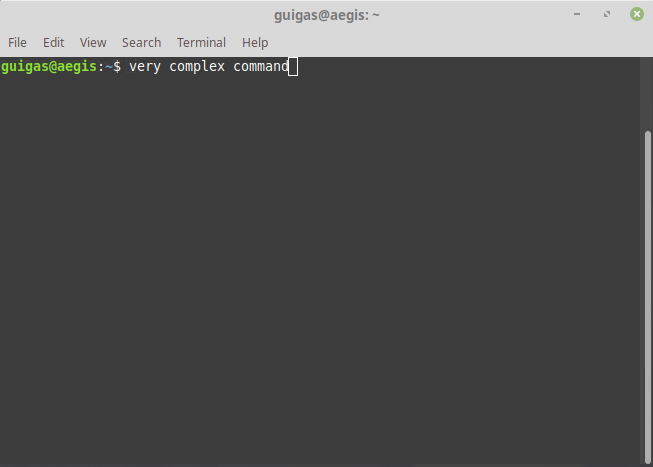
\includegraphics[width=\linewidth]{term2.png}
		\caption{A figura mostra a interface gráfica de um terminal atual.}
		\label{fig:term1}
	\end{figure}
	\subsection{Console}
	Então, terminal é um meio de acesso a um console, mas os comandos que você insere também não são do console, e sim do Shell, mas voltando ao console, não é necessário um terminal para acessar um console. Em um sistema linux, apertando "ctrl" + "alt" + "F1 , F2 , ... , F6" é possível acessar um dos consoles (F7 para sair). Hoje, isso também é conhecido como o modo texto do seu sistema operacional, pois é mais intuitivo que usar o termo console. Se um terminal era uma estação com tela e teclado, o console era a conexão física e digital entre o terminal e o mainframe. Então, Para cada sistema existe um console diferente, ligando cada sistema, a uma interface (geralmente, de texto), existem diferentes consoles que servem como interfaces para diferentes sistemas: BIOS, Boot Loader, init (processo incial do boot de sistemas unix). O console que está em uso quando você usa um terminal te da acesso ao Shell.
	\subsection{Shell}
	Shell possui esse nome pois ele funciona como uma casca separando o kernel do exterior. Sua função é servir de interface para acessar as funções do sistema operacional, tendo a vantagem de funcionar da mesma maneira em qualquer sistema operacional baseado em unix, escondendo detalhes específicos de cada SO.
	\begin{figure}[h]
		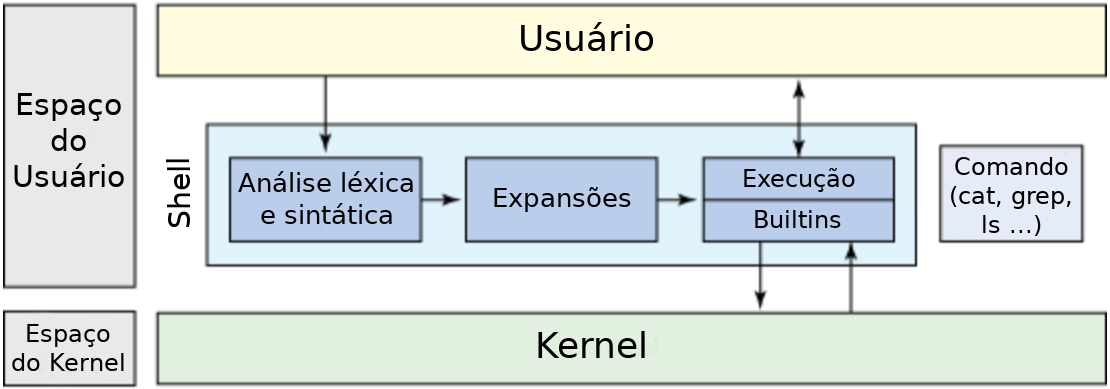
\includegraphics[width=\linewidth]{shell_struct1.png}
		\caption{A figura detalha como o Shell faz a interação entre o Usuário e o Kernel.}
		\label{fig:shellstruct}
	\end{figure}\\
	Portanto, os comandos inseridos no terminal são programas (arquivos executáveis) executados pelo Shell em uso, que, na maioria dos sistemas linux atualmente, é o Bash. Diferentes Shells possuem funcionalidades diferentes, essas funcionalidades incluem:
	\begin{itemize}
		\item Executar comandos.
		\item Manipulação de diretórios.
		\item Controle de processos (jobs).
		\item Expansões.
		\item Redirecionamento.
		\item pseudônimos (aliases).
		\item Histórico de comandos.
	\end{itemize}
	E muitas outras funcionalidades para facilitar, agilizar e automatizar as atividades realizadas.\\
	Essas são algumas funcionalidades que estamos acostumados a utilizar hoje, mas nas primeiras versões de Shell, muitas delas não existiam.
	
	\section{Unix, GNU e Shell}
	Em 1971, Ken Thompson desenvolveu o primeiro UNIX Shell, chamado de V6 Shell (foi criado no Unix versão 6), com funcionalidades muito básicas, ele permitia pipes e redirecionamentos, mas era um interpretador de comandos, ao invés de scripts.
	
	Apenas executar comandos e redirecionamento de entrada e saída não eram o suficiente para a necessidade dos usuários, além de que a interface não facilitava atividades repetitivas. Dessa necessidade surgem novos Shells, com novas funcionalidades. Em 1977 foi criado o Bourne Shell, com dois objetivos: Servir como um interpretador de comandos e executar scripts. Além disso, o Bourne Shell acrescentou ferramentas de controle (até então "if" existia como uma extensão, mas não era implementado diretamente no Shell V6), loops e variáveis, facilitando o uso de comandos e a criação de scripts. A partir disso surgem muitos outros Shells, e todos seguiram essas funcionalidades. Os principais foram: C-Shell, com o objetivo de deixar os scripts mais parecidos com a linguagem C. Korn Shell, que adicionou novas funcionalidades ao mesmo tempo que manteve forte compatibilidade com o Bourne Shell, e por fim, o Bourne Again Shell (Bash), que além de manter a compatibilidade com o Bourne Shell, também implementou as funcionalidades do C-Shell e Korn shell, ele também continuou a evoluir com o tempo, porém, um dos grandes facilitadores para o Bash ser o mais usado dos 3 é o fato de ele ser um projeto Open Source do GNU.
	
	O projeto GNU (GNU is Not Unix) não se trata apenas de criar uma versão open source do UNIX, mas sim de criar um ambiente onde sistemas abertos respeitam especificações e padrões, de modo que os usuários tivessem a liberdade para escolher, usar, distribuir e modificar software, e para isso é necessário que todo o sofware, incluíndo SO, drivers e programas fossem software livre. Para isso a criação do Bash foi necessária, e com o sucesso do Manifesto GNU \cite{gnu}, o Bash foi o Shell mais difundido.
	
	\section{Z shell}	
	Ainda existem Shells sendo criado até hoje, geralmente adicionando funcionalidades para facilitar o uso das ferramentas já existentes no Bash, por exemplo, o Z shell (zsh) permite que usuário selecione o resultado das expansões de nomes de arquivos antes de executar o comando, além disso, quando o usuário digita parte de um caminho da árvore de diretórios, o zsh deixa visível os arquivos e diretórios visíveis à partir do caminho digitado, assim, unindo a intuitividade da interface gráfica com a agilidade da interface textual. 
	
	\section{Conclusão}
	A maior evolução de qualquer Unix Shell foi a ideia de transformar o shell em uma ferramenta para Scripts, e não apenas um interpretador de comandos, essa mudança surgiu no Bourne Shell, e é bem provável que, qualquer que seja o Shell mais comum no futuro, continue sendo algum derivado do Bourne Shell.
	
	\part{Bash Básico}
	
	\section{Comandos em Bash}
	Se você já precisou usar comandos do Bash para buscar partes específicas de um arquivo de texto, você sabe que muitas vezes é necessário usar mais de um comando, e simplesmente não é prático usar vários arquivos intermediários para chegar no seu resultado final. O próximo parágrafo desse material explica como usar qualquer comando, porém, o Bash não se tornou o Shell mais utilizado por ser um simples interpretador de comandos. As próximas seções explicam o sistema de arquivos e diretórios e maneiras de navegar entre eles, além do uso de pipelines, expansões e ferramentas de entrada e saída para usar o Bash como um interpretador de scripts, e não apenas de comandos separados.
	
	\section{Estrutura do Bash}
	Uma linha de comando consiste de uma ou mais palavras, separadas por espaços. A primeira palavra é o próprio comando, seguido de um ou mais parâmetros(alguns comandos não exigem nenhum parâmetro). Um tipo comum de parâmetros são as opções, geralmente na forma de um traço seguido de uma letra. Algumas opções têm seus próprios parâmetros. Para exemplificar, vamos usar um comando que ordena linhas, o "sort". Suponha que queremos ordenar as linhas de um arquivo chamado lista.txt e queremos uma ordenação numérica, para isso usamos o seguinte comando: \texttt{\textbf{\textit{sort -n lista.txt}}}.
	Neste caso, "sort" é o comando, "-n" é a opção que indica ordenação numérica e o "lista.txt" é o parâmetro que seleciona qual arquivo deve ser ordenado.
	Para saber quais opções e quantos parâmetros um comando pode ter, utilize o comando man, que também detalha o funcionamento do comando, então, em caso de dúvidas sobre como usar algum comando, leia a man page. basta digitar: \texttt{\textbf{\textit{man comando}}}, trocando "comando" pelo comando a ser consultado.
	Neste caso, "man" é o comando e "comando" é o parâmetro para escolher qual man page deve ser consultada.
	
	\subsection{Arquivos e Diretórios}
	Em sistema UNIX, o conceito de arquivo é bem amplo, não há nenhuma estrutura definida, o significado da sequência de bytes armazenada em um arquivo, é dependente de qual aplicação o utiliza. O nome do arquivo também não é definido. Todo tipo de padrão como headers, conteúdo e extensões(".txt, .mp3") são maneiras de organizar os arquivos. É possível separar os tipos de arquivos em 3:
	\begin{itemize}
		\item Arquivo de texto, que contém caracteres legíveis.
		\item Arquivo executável, o conteúdo desse tipo de arquivo não são caracteres legíveis, então não é uma boa ideia abrir um arquivo como esse em um editor de texto.
		\item Diretório. Conhecidos pela abstração "pasta". São criados para guardar outros arquivos (qualquer tipo, até outros diretórios).
	\end{itemize}
	\subsection{Navegação}
	Uma abstração importante dos sitemas UNIX é a árvore de diretórios. Mesmo que os dados não sejam armazenados dessa forma, diretórios possuem uma estrutura hierárquica, onde um diretório é o pai de todos os diretórios que ele contém. Diretórios são irmãos, se possuem o mesmo pai, além disso, diretórios possuem apenas um pai. O diretório raiz é chamado "root".
	
	Para poder navegar pela árvore de diretórios e não precisar saber ou digitar o caminho completo de um arquivo, existe o conceito de diretório atual, assim, é possível se referir a arquivos tanto de maneira relativa a esse diretório quanto de maneira absoluta(partindo do root, para isso, o caminho deve começar com uma barra (/)). Os caminhos são compostos de diretórios separados por barra. Para que um caminho seja válido, os diretórios em sequência, devem possuir uma conexão na árvore de diretórios.
	
	Além disso, Todo diretório possui uma conexão ao diretório pai (..) e a si mesmo (.), assim, é possível acessar qualquer diretório, a partir de qualquer outro diretório, porém, caso o diretório corrente seja um diretório profundo de um ramo da árvore, pode ser mais rápido acessar o diretório desejado pelo seu caminho absoluto, partindo da raiz, ao invés de retornar vários diretórios usando "..".
	
	Além da árvore de diretórios e do diretório atual, no UNIX, cada usuário possui um diretório "home", esse diretório serve para separar os arquivos do sistema, executáveis de programas, e outros arquivos, dos diretórios pessoais do usuário. Convenientemente, um usuário logado possui um atalho para a sua home, sendo assim, ele sempre pode se referenciar a sua home com o caractere TIL (\texttildelow).
	Exemplos: 
	\begin{lstlisting}
	/home/usuario/Documentos
	../../media/dispositivo
	~/Downloads
	\end{lstlisting}
	Os comandos da tabela \ref{table:1} são os mais usados para navegação na árvore de diretórios:
	
	\begin{table}[!ht]
		\centering
		\begin{tabular}{ | c | c | } 
			\hline
			\bfseries Nome do comando & \bfseries Função \\
			\hline
			pwd & Retorna o diretório atual \\
			\hline
			ls & Lista os arquivos de um diretório \\
			\hline
			cd & Muda o diretório atual \\
			\hline
			mkdir & Cria um novo diretório \\
			\hline
		\end{tabular}
		\caption{A tabela explica o funcionamento dos comandos básicos de navegação}
		\label{table:1}
	\end{table}
	O comando ls pode ser usado no diretório atual ao omitir o parâmetro de localização, existem opcionais para mostrar metadados e incluir arquivos ocultos (arquivo cujo nome começa com ponto (.)). O comando cd aceita tanto caminho absoluto quando caminho relativo. Ao omitir o parâmetro de localização o diretório atual será a home. Mais detalhes sobre as opções e parâmetros dos comandos podem ser encontrados nas man pages. O mesmo vale para os comandos apresentados até o fim desse material. É indicado que o leitor teste o que é apresentado nesse material, lendo as man pages e testando opções dos comandos.
	
	Dica: Utilize o auto-complete para evitar digitação desnecessária! TAB para completar quando há apenas uma opção possível e TAB duas vezes para mostras as opções possíveis, tanto para completar comandos quanto para nomes de arquivos e diretórios existentes e acessíveis no caminho digitado(na verdade, os comandos também são arquivos, os comandos do Bash ficam no diretório /bin).
	
	\section{Bash para scripts} \label{scripts}
	
	A seção anterior detalha como navegar na árvore de diretórios, porém, muitas vezes não mantemos um mapa mental completo da árvore e nesse caso a navegação, mesmo com auto-complete ainda é muito precária para escrever comandos para vários arquivos. Para facilitar esse trabalho, usa-se caracteres coringas, ou, "meta-caracteres".
		
	\subsection{Expansão}
	
	O asterísco (*) substitui qualquer sequência de caracteres e o ponto de interrogação (?) substitui um único caractere. Então, suponha que em seu diretório atual, existem os seguintes arquivos: b16c8a16.txt, b4c4a32.txt e b128c2a8.txt, suponha também uma infinidade de arquivos com nomes variados de modo que ls não é a forma mais rápida de identificar arquivos. com o asterísco, é possível selecionar um arquivo sabendo apenas parte de seu nome, por exemplo, o comando "ls b16*" retornaria apenas o arquivo b16c4a32.txt (caso nenhum outro arquivo do diretório corrente comece com b16). o comando "ls b1?c" retorna apenas o arquivo b16c8a16.txt. Usando um "*" no lugar do "?", o comando retornaria tanto o arquivo "b16c8a16.txt" quanto o "b128c2a8.txt".
	
	Suponha agora que você quer imprimir o conteúdo de todos os arquivos que acabam em ".txt". O comando cat imprime o conteúdo de um arquivo na tela. Caso o usuário não saiba o nome de todos os arquivos(ou apenas não queira digitar todos), mesmo que sejam muitos arquivos, ainda é possível realizar essa tarefa apenas com o seguinte comando:
	\begin{lstlisting}
	cat *.txt
	\end{lstlisting}
	Com os comandos mv(mover) e cp(copiar) é possível realizar rapidamente tarefas bem comuns de gestão de arquivos. É indicado que o leitor crie um diretório para testar comandos com '*' e '?', em especial com o comando rm (remover). Cuidado com o uso de ".*", lembre dos diretórios . e .. antes de executar comandos destrutivos.
	
	Com o uso dos colchetes ('[' e ']') é possível criar coringas mais específicos para a expansão de caminhos, por exemplo, a expansão *.[abc] funciona para todos os 3 casos: "*.a", "*.b" e "*.c". A tabela \ref{table:2} possui mais exemplos de expansão, lembre que a expansão de colchetes corresponde a um único carectere:
	\begin{table}[!ht]
		\centering
		\begin{tabular}{ | c | c | } 
			\hline
			\bfseries Expansão & \bfseries corresponde à \\
			\hline
			[b-e.;!] & Qualquer letra minúscula de "b" a "e", ".", ";" e "!" \\
			\hline
			[!b-e] & Qualquer dígito, exceto letras minúsculas de "b" a "e" \\
			\hline
			[A-Z0-9] & Qualquer letra maiúscula de "A" a "Z" e qualquer número de um dígito \\
			\hline
			[a-df-i] & a, b, c, d, f, g, h, i \\
			\hline
			[abc-] & 'a', 'b', 'c', ou '-' \\
			\hline
		\end{tabular}
		\caption{A tabela descreve o resultado de alguns exemplos de expansão}
		\label{table:2}
	\end{table}
	
	Expansão de caminhos é o primeiro passo para fazer scripts em Bash, com eles é possível realizar ações para várias entradas, de uma só vez. Porém, nem todo parâmetro é um nome de arquivo ou diretório, para isso existe a expansão de chaves ('\{' e '\}'), que permite a expansão para um conjunto de strings, separadas por ','. Apesar de funcionar de maneira parecida, nesse tipo de expansão, não há a necessidade de corresponder com nomes de arquivos existentes. A tabela \ref{table:3} contém exemplos de uso da expansão de chaves:
	
	\begin{table}[!ht]
		\centering
		\begin{tabular}{ | c | c | } 
			\hline
			\bfseries Expansão & \bfseries Resultado \\
			\hline
			cat func.\{c,h\} & conteúdo dos arquivos fun.c func.h \\
			\hline
			ls rec0\{1..4\}.mp3 & rec01.mp3 rec02.mp3 rec03.mp3 rec04.mp3 \\
			\hline
			\multirow{2}{13em}{touch 201\{5..7\}/ex\{1..4\}.txt} & cria ex1.txt, ex2.txt, ex3.txt e ex4.txt \\ 
			& nos diretórios 2015, 2016 e 2017 \\
			\hline
			echo turma\{A..D\} & turmaA turmaB turmaC turma D\\
			\hline
			echo turma\{A..G..2\} & turmaA turmaC turmaE turma G\\
			\hline
		\end{tabular}
		\caption{A coluna direita descreve o resultado do comando da coluna esquerda}
		\label{table:3}
	\end{table}
	Se necessário, consulte as man pages dos comandos echo e touch. Com a expansão de chaves é possível expandir caminhos que não existem, então dependendo do caso você pode obter respostas de erro do comando utilizado.
	
	As mensagens de erro dos comandos do Bash são bem intuitivas, antes de ir ao google, leia a mensagem de erro, e se necessário a man page. Para os casos comuns, isso basta.
	
	Em caso de dúvidas nos resultados das expansões, use o comando echo para conferir se a expansão gera o resultado esperado, antes de usar a expansão em comandos que podem estragar ou mover arquivos importantes. Lembre-se da diferença entre a expansão de chaves da expanção de colchetes.
	
	\subsection{Redirecionamento de Entrada e Saída}
	
	Os redirecionamentos são o próximo passo da evolução de comandos para scripts. As expansões são muito úteis, mas nem tudo pode ser resolvido com apenas um comando. Uma ótima abstração para entender a funcionalidade do redirecionamento no Bash é pensar nos comandos como filtros. Um comando recebe uma entrada e produz uma saída, até esse ponto do material a entrada era sempre lida pelo teclado (stdin - Standard Input) e imprimidas na tela (stdout - Standard Output), porém, se é possível usar comandos como filtros, podemos redirecionar a saída de um comando para a entrada de outro, e assim, combinar vários comandos para obter a saída desejada, com uma estrutura parecida com esta:
	
	\begin{lstlisting}
	entrada -> Filtro1 -> Filtro2 -> ... -> FiltroN -> saída
	\end{lstlisting}
	A notação para redirecionamento de entrada é '<' e, '>' para saída. Então, o seguinte exemplo redireciona a saída do comando cat para o arquivo teste.txt:
	
	\begin{lstlisting}
	cat texto.txt > teste.txt
	\end{lstlisting}
	Também é possível redirecionar a entrada de um comando. Suponha um programa que lê na entrada padrão. Caso hajam muitas entradas de teste ou caso a entrada seja muito grande. É possível redirecionar um arquivo como entrada dessa forma:
	
	\begin{lstlisting}
	./programa < entrada1.txt
	\end{lstlisting}
	Observação: './' é a maneira de executar um arquivo executável (tente './ls' no diretório '/bin').
	
	A última ferramente para usar programas e comandos como filtros, como exemplificado anteriormente é o pipeline (|). O pipeline elimina a necessidade de arquivos intermediários e liga diretamente a saída de um programa a entrada de outro conforme o exemplo:
	
	\begin{lstlisting}
	ls /dev | grep std | tee file1.txt file2.txt file3.txt
	\end{lstlisting}
	O resultado desse comando imprime 3 arquivos: 'stdin', 'stdout' e 'stderr'. O terceiro ainda não foi apresentado nesse material. stderr é, por convenção, o local para imprimir warnings e erros dos programas, como um log.
	O comando grep seleciona apenas as linhas do resultado que contém a substring passada como parâmetro. O comando tee redireciona a entrada para todos os arquivos passados como parâmetro.
	
	Um uso comum do pipeline é filtrar diferentes dados dos nomes de arquivos partindo do comando ls, ou do conteúdo desses, partindo do comando cat, e utilizar os comandos grep, cut e tr, respectivamente para filtrar linhas específicas, filtrar seções de uma linhas e substituir caracteres, e, ao final é possível redirecionar a saída para um arquivo.
	
	\section{Exercício}
	
	\begin{enumerate}
		\item Utilizando apenas um comando mkdir e expansão de chaves, crie os 7 diretórios com os seguintes nomes: 3 diretórios para turmaAP, turmaREP e turmaFN e os 3 diretórios turmaA, turmaB e turmaC 1 diretório de nome alunos. Dentro de um diretório seguro para testes.
		
		Resposta:
		\begin{lstlisting}
		mkdir turma{{A..C},{AP,REP,FN}} alunos
		\end{lstlisting}
		\item dentro do diretório alunos, crie arquivos de nome de alunos no formato aluCnotaN para cada curso C entre: BCC, IBM, TADS e OUTRO e para cada nota N entre 0 a 10 e NULL. Exemplo de arquivo: aluBCCnotaNULL
		
		Resposta:
		\begin{lstlisting}
		touch alunos/alu{BCC,IBM,TADS,OUTRO}nota{{0..10},NULL}
		\end{lstlisting}
		\item Copie os arquivos do diretório alunos para o diretório correspondente de acordo com a tabela \ref{table:4}:
		
		\begin{table}[!ht]
			\centering
			\begin{tabular}{ | c | c | c | } 
				\hline
				\bfseries Exercício & \bfseries Arquivos & \bfseries Copiar para \\
				\hline
				3.1 & Alunos de BCC com nota diferente de NULL & turmaA \\
				\hline
				3.2 & Alunos de IBM com nota diferente de NULL & turmaB \\
				\hline
				3.3 & Alunos de TADS com nota diferente de NULL & turmaC \\
				\hline
				3.4 & Alunos de BCC, IBM e TADS com nota de 0 a 3 & turmaREP \\
				\hline
				3.5 & Alunos de BCC, IBM e TADS com nota de 4 a 6 & turmaFN \\
				\hline
				3.6 & Alunos de BCC, IBM e TADS com nota de 7 a 10 & turmaAP \\
				\hline
			\end{tabular}
			\caption{Relação do destino dos arquivos para o exercício 3}
			\label{table:4}
		\end{table}
		Resposta:
		\begin{lstlisting}
		cp alunos/aluBCCnota[!A-Z]* turmaA/
		cp alunos/aluIBMnota[!A-Z]* turmaB/
		cp alunos/aluTADSnota[!A-Z]* turmaC/
		cp alunos/alu{BCC,IBM,TADS}nota[0-3] turmaREP/
		cp alunos/alu{BCC,IBM,TADS}nota[4-6] turmaFN/
		cp alunos/alu{BCC,IBM,TADS}nota{7..10} turmaAP/
		\end{lstlisting}
	\end{enumerate}
	
	\section{Conclusão}
	As ferramentas do Bash apresentadas nesse material, juntamente com estruturas de controle (if e for) e variáveis, permitem que sejam criados scripts que interagem dinamicamente com os dados sem excesso de digitação e trabalho por parte do usuário. Para que esse conteúdo seja entendido pelo leitor é ideal que os conhecimentos sejam aplicados na prática. Para isso, são indicados os materiais do professor Roberto Hexsel \cite{roberto1, roberto2}, que, além de serem bem explicativos, possuem vários exemplos, explicam novos comandos e contém alguns exercícios para praticar.
	
\bibliographystyle{apalike}
\bibliography{artbib}

%----------------------------------------------------------------------------------------
%	REFERENCE LIST
%----------------------------------------------------------------------------------------
\end{document}
